\section{Experiments}
We conducted several experiments to study the scalability of our solution. Firstly we study the throughput and mean message latency variation with the number of \textit{QueryEvaluators} for both single JVM and distributed setups. In an ideal system, we should observe linear throughput increment with a constant message latency. However there are some exceptions and we have provided our explanations on them. Finally we study the throughput variation with the window size to study the suitability of our solution for higher window sizes. All these experiments were performed on a LAN with a network bandwidth of 1Gbps and all machines were Intel(R) Xeon(R) 2.4GHz, 4 core duo machines with 16 GB of memory. 

\subsection{Frequent routes query}

\begin{figure}[!t]
        \centering
        \includegraphics[width=3.0in]{routegraph.png}
        \caption{Process graph to evaluate top ten frequent routes.}
        \label{routegraph}
\end{figure}

Figure \ref{routegraph} shows the process graph used to process frequent route queries. \textit{RouteEventEmitter} reads the data file and emits events with a sequence number. \textit{RouteEmitter} contains a set of threads (equals to the number of \textit{RouteProcessors}) to emit events more efficiently. When processing each line first it reads the data line and creates a \textit{Route} object using longitude and latitude coordinates of pickup and dropoff locations. Then it distributes the events among the \textit{RouteProcessors} using the hash value of the \textit{Route} object. \textit{TopRouteProcessor} aggregates the results and saves them to a file.

We deployed this process graph to a distributed stream processing system we have developed, and  measured the throughput and the mean message latency varying the number of \textit{RouteProcessors} with the data set given (173 million records). In the local set up, we use a new thread to execute a new instance and in the distributed setup we add a new node to execute the new instance.

\begin{figure}[!t]
        \centering
        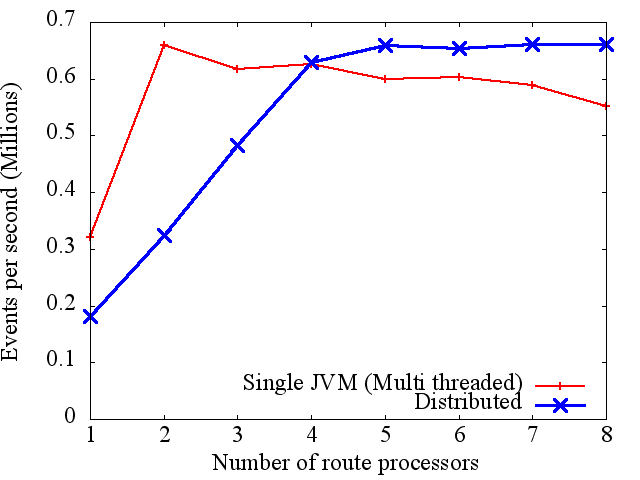
\includegraphics[width=3.0in]{throughput_route.png}
        \caption{Throughput variation with the number of \textit{RouteProcessor} instances.}
        \label{throughput_route}
\end{figure}

Figure \ref{throughput_route} shows the throughput variation. For single JVM setup throughput increases from one instance to two instances. This is due to higher parallelism system achieves with two threads. After that throughput slightly decreases due to higher context switching with many threads. Similarly for distributed setup initially throughput increases with the number of   \textit{RouteProcessors} and achieves a steady limit. We observe two reasons for this non scalability after initial stages. Firstly, \textit{RouteProcessor} is not a computing intensive process. Secondly, there is only one \textit{RouteEventEmitter} and the speed at which it can read and send messages becomes the bottleneck. Initial throughput for distributed setup is less, due to message serialization, message deserialization and tcp overheads. 

\begin{figure}[!t]
        \centering
        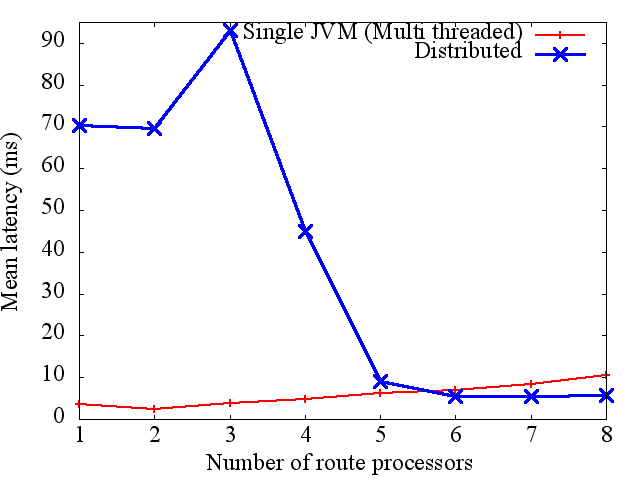
\includegraphics[width=3.0in]{latency_route.png}
        \caption{Mean latency variation with the number of \textit{RouteProcessor} instances.}
        \label{latency_route}
\end{figure}

Figure \ref{latency_route} shows the latency variation. For single JVM setup latency get reduced at 2 and slightly increases after that due to context switching overhead with higher number of threads. For distributed setup there is an high initial latency due to communication overheads. After that it comes to a constant value. 

\subsection{Profitable cells query}

\begin{figure}[!t]
        \centering
        \includegraphics[width=3.0in]{profictgraph.png}
        \caption{Process graph to evaluate top ten profitable cells.}
        \label{profictgraph}
\end{figure}

Figure \ref{profictgraph} shows the process graph for profitable cells query. \textit{ProfitEventEmitter} reads the data file and calculates the pickup cell and dropoff cell details using longitude and latitude coordinates. Then it creates two events one for dropoff part and other to pickup part, with different sequence numbers and distributes the events among \textit{ProfitCalculators} using the hash value of the cell. In this way cells are partitioned into different \textit{ProfitCalculator} instances and each instance gets all the events relevant to its' cell set. We use a set of threads (equals to the number of Profict Calculators) to emit data as in the previous query. Finally \textit{TopProfitProcessor} aggregates events and writes to a file. 

Similar to earlier experiment,  we deployed this process graph to our system and measured the throughput and the average message latency increasing the number of  \textit{ProfitCalculaor} instances for both single JVM setup and distributed setup to examine the scalability of our solution.

\begin{figure}[!t]
        \centering
        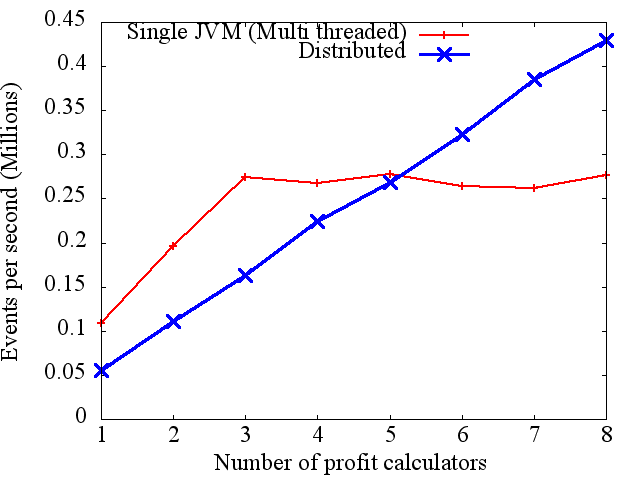
\includegraphics[width=3.0in]{throughput_profit.png}
        \caption{Throughput variation with the number of \textit{ProfitCalculator} instances.}
        \label{throughput_profit}
\end{figure}
 
Figure \ref{throughput_profit} shows the throughput variation for both setups. For single JVM set up initially throughput increases, due to increment of parallelism and comes to a steady state. For distributed setup  throughput increases linearly, although it has an initial lesser throughput compared to single JVM setup due to message serialization, message deserialization and tcp overheads. 

\begin{figure}[!t]
        \centering
        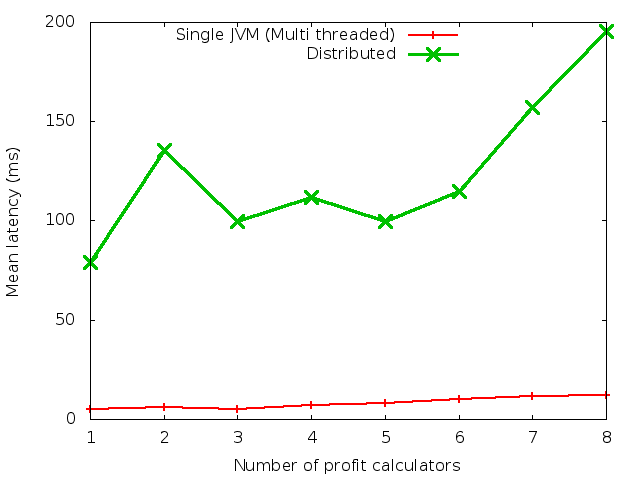
\includegraphics[width=3.0in]{latency_profit.png}
        \caption{Mean latency variation with the number of \textit{ProfitCalculator} instances.}
        \label{latency_profit}
\end{figure}

Figure \ref{latency_profit} shows the latency variation for both setups. For single JVM, latencies slightly increased with the addition of new instances as expected. But for distributed setups latency linearly increases with the addition of new nodes after 6 \textit{ProfitCalculator} instances. This latency increment is due to longer queues at the \textit{TopProfitProcessor}. In our message ordering process, we can send a message to \textit{TopProfitProcessor} only if all queues are not empty. This allows some processes with less top ten profitable events to delay other process messages. This problem can  possibly fixed by adding a limit to the message queue size. On the other hand in a real time system, this event ordering many not required since event processing happens at real time.

\subsection{Scalability with Window Size}

The grand challenge problem uses 15 minute window size for profitable cells query. However in a real world problems window sizes may required. Therefore finally we evaluated scalability of our solution with the window size.  For this experiment, we measured the throughput of the profitable cells query using a single JVM and three instances by varying the window size. Further we compared the throughput with our \textit{DynamicHeap} based solution which is not effective in lower window sizes as well.

\begin{figure}[!t]
        \centering
        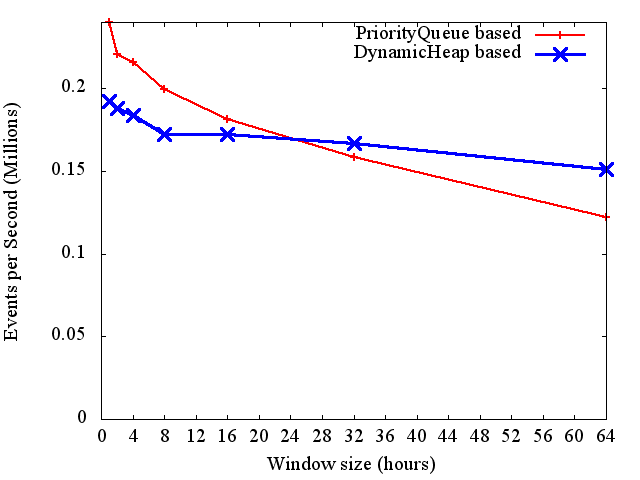
\includegraphics[width=3.0in]{window.png}
        \caption{Throughput variation with the window size.}
        \label{window}
\end{figure}

Figure \ref{window} shows the results. For both solutions, throughput does not drop by half, even though the window size increases 64 times. And for large windows \textit{DynamicHeap} performs better than the \textit{PriorityQueue} based one. This is due to two reasons. Firstly, all operations of \textit{DynamicHeap} are O(log(n)). Secondly, out of 173 million records there are only around 18000 unique fares. Therefore \textit{DyamicHeap} based algorithm does not consume memory beyond that. However , since \textit{PriortyQueue} based implementation keeps all values in memory it consumes more memory for large windows.
